\documentclass{article}

\usepackage[top=1in,bottom=1in,left=1in,right=1in]{geometry}
\usepackage{color}
\usepackage{graphicx}
\usepackage{amsmath}
\usepackage{float}
\usepackage{booktabs}
\usepackage{indentfirst}
\usepackage{textcomp}
\usepackage{enumerate}
\usepackage{float}
\usepackage{url}
\usepackage{setspace}
\usepackage{multirow}
\usepackage{chngpage}
\usepackage{array}
\usepackage{amssymb}
\usepackage{subfig}
\usepackage{bm}
\usepackage{mathrsfs}
\usepackage{listings}
\usepackage{xcolor}
\usepackage{algorithm}
\usepackage[noend]{algpseudocode}
\lstset{
	numbers=left, 
	numberstyle= \tiny, 
	keywordstyle= \color{ blue!70},
	commentstyle= \color{red!50!green!50!blue!50}, 
	frame=shadowbox,
	rulesepcolor= \color{ red!20!green!20!blue!20} ,
	escapeinside=``, 
	xleftmargin=2em,xrightmargin=2em, aboveskip=1em,
	framexleftmargin=2em,
	showstringspaces=false, % not showing space
	breaklines=true,
	tabsize=4,
	stringstyle=\ttfamily,
}
 
\usepackage[numbers]{natbib}
\citestyle{IEEEtran}
\bibliographystyle{IEEEtranN}

\title{EECS 442 Final Project - License Plate Recognition}
\author{Jiongsheng Cai\\
			Jingyao Hu\\
			Yucheng Yin}
\begin{document}

\maketitle
\begin{spacing}{1.0}
\section{Introduction}
Automatic License Plate Recognition (ALPR) has become a popular technology since it was invented in 1976 at the Police Scientific Development Branch in the UK \cite{wikipedia_ANPR}. It can be used in different fields like checking whether a vehicle is registered or licensed by police forces, or used for pay-per-use roads like electronic toll collection and parking lot. Our group tries to solve the license plate recognition problem by following a classical series of steps. That is, plate localization and extraction, segmentation, and finally character recognition by CNN.

\section{Related Work}
Since the technology has been invented for over 40 years, there are quite a lot of well-implemented tools and libraries available. Our goal is not to directly use these well-developed tools but to implement our own version of LPR and most importantly, deepen our understanding of the typical algorithm. We searched online for typical algorithms and find generally two sets. 

\subsection{Classic Method}
As mentioned in the relatively earlier papers \cite{toda2005license}, a typical process of license recognition could include:
\begin{itemize}
	\item \textbf{Plate localization and extraction.}
	
	\item \textbf{Character segmentation.}
	
	\item \textbf{Recognition.}
\end{itemize}

\subsection{Methods utilizing Neural Networks}
As the development of Neural Networks these years, there have been a lot of NN-related methods to solve License-plate recognition problems \cite{Wu2017}. Compared with the classic methods, the NN-related methods have a faster processing speed and higher accuracy in recognition.

\section{Methods}
Our method is based on the classic model of LPR and utilize the basic techniques we have learned in EECS442. Some of the procedures have been simplified due to the time limit and all the key components of the algorithm are implemented by ourselves.

\subsection{Dataset}
There are a few dataset for license plates online but some of them are significantly variant in terms of illumination, viewing angle and plate structure, which will cause great difficulty to our project. Therefore, we choose a relatively well-built dataset. Note that the dataset doesn't come with labels which cause us difficult to manually count the accuracy of recognition due to the relatively large size of the dataset.

\subsection{License Plate Localization and Extraction}
\begin{itemize}
	\item \textbf{Edge Detection} Before we start to find the plate location, we need to remove unnecessary information from the image. Although MATLAB has built-in functions for achieving such goals, we implemented our own version of edge detection which utilizes the sobel filter. In short, we apply two matrix
	$$
	S_x =
	\begin{bmatrix}
	-1 & -2 & -1 \\
	0 & 0 & 0 \\
	1 & 2 & 1
	\end{bmatrix}
	~~
	S_y = 
	\begin{bmatrix}
	-1 & 0 & 1 \\
	-2 & 0 & 2 \\
	-1 & 0 & 1
	\end{bmatrix}
	$$
	on the original image to calculate the strength at each pixel and after normalization, we convert the gray-scale image to a black-and-white image with edges detected.
	
	\item \textbf{Histogram variation} After the edge detection, we calculate the horizontal and vertical histogram. For the horizontal histogram, it's calculated by traversing each column of the image. It starts traversing with the second pixel form the top of each column and the difference between second and first pixel is calculated. In the meantime, we maintain a sum value for each column. If the difference is greater than a threshold, it is added to the total sum of differences. In the end, we get an array for column wise sum. The vertical histogram is calculated exactly same as horizontal histogram.
	
	\item \textbf{Image cropping} After we get the two histograms, we start to find the horizontal and vertical location of the license plate. Take horizontal location as an example. We maintain a starting point and an end point while traversing the horizontal histogram array. If certain value is greater than pre-defined threshold, we mark it as starting point and continue until certain value is smaller than threshold, then we mark it as end point. Therefore we will get many pairs of staring and ending points. We choose the pair with largest difference (length). The process for finding vertical location is the same story. 
	
\end{itemize}

\subsection{Character Segmentation}
\begin{itemize}
	\item After we get the extracted plate, we need to segment each character of the plate for the recognition. We take the advantage of the large color difference (black and white) between the character and the space in the middle of two characters. The following is the specific description of the algorithm. 
	\begin{algorithm}
	
		\begin{algorithmic}[1]
			\Procedure{Segment}{}
			\State $start\_position = 0$
			\For{i:column(image)} 
			\State Record the position when we fully pass a character
			\State Record the position when we meet the second character
			\State Reset the start position and flags
			\EndFor
		
			\EndProcedure
		\end{algorithmic}
	\end{algorithm}
 \item After we get the raw segmentation, we further remove the noise by utilizing the factor that the ratio of white weight to black and the ratio of column to row are in some specific range for the characters we want. Therefore, we manage to filter out some noisy segmented results.
\end{itemize}

\subsection{Character Recognition}
\begin{itemize}
	\item After we get the exact segmentation for each character in the license plate. We decided to implement a character-level character recognition. Our work is based on a convolutional neural network (CNN) trained on EMNIST dataset \cite{DBLP:journals/corr/CohenATS17}. EMNIST dataset is an extension of MNIST dataset, which shares the same image structure and parameters as the original MNIST task, involving handwritten letters (uppercase and lowercase) and digits.
	\item  We chose to train our network on balanced classes, which contains 131,600 characters and 47 balanced class. Considering computational efficiency, we implemented a common and simple network structure for MNIST training. For image pre-processing, we resize every image (of character segmentaion) into 28*28. The network structure follows as two 3*3 convolutional layers, one max-pooling layer, and one fully-connected layer. We use softmax funcion for multiple classes classification. 
	\item Our network shows an accuracy of 87.33\% on EMNIST test data. 
	
\end{itemize}

\section{Results}
As mentioned above, our dataset doesn't come with labels. Due to the large size, we don't count manually to calculate the accuracy for these plate numbers. By our observation, we find that the plate extraction and character segmentation is quite good, while the character recognition is relatively poor, which causes the recognition accuracy relatively low. We will present one set of good example and one set of bad example. The reason for good or bad recognition will be discussed in the following section.

\begin{itemize}
	\item One good example.
	\begin{figure}[H]
		\centering
		\begin{minipage}{5cm}
			
\includegraphics[width=5cm]{P1010003.jpg}
			\caption{Original Image}
		\end{minipage}
		\begin{minipage}{5cm}
			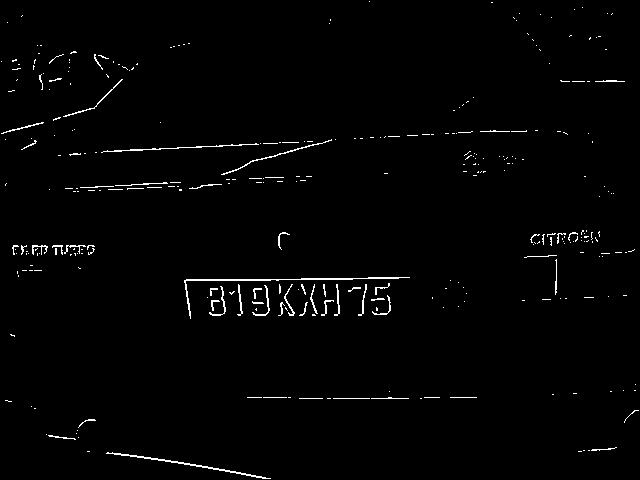
\includegraphics[width=5cm]{P1010003_edge.jpg}
			\caption{After edge detection}
		\end{minipage}
		\begin{minipage}{5cm}
			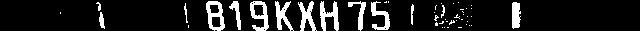
\includegraphics[width=5cm]{P1010003_extract.jpg}
			\caption{After segmentation}
		\end{minipage}
	\end{figure}

	\begin{figure}[H]
		\centering
		\begin{minipage}{0.7cm}
			
\includegraphics[width=0.7cm]{P1010003_0.jpg}
		\end{minipage}
		\begin{minipage}{0.7cm}
			
\includegraphics[width=0.7cm]{P1010003_1.jpg}
		\end{minipage}
		\begin{minipage}{0.7cm}
			
\includegraphics[width=0.7cm]{P1010003_2.jpg}
		\end{minipage}
		\begin{minipage}{0.7cm}
			
\includegraphics[width=0.7cm]{P1010003_3.jpg}
		\end{minipage}
		\begin{minipage}{0.7cm}
			
\includegraphics[width=0.7cm]{P1010003_4.jpg}
		\end{minipage}
		\begin{minipage}{0.7cm}
			
\includegraphics[width=0.7cm]{P1010003_5.jpg}
		\end{minipage}
		\begin{minipage}{0.7cm}
			
\includegraphics[width=0.7cm]{P1010003_6.jpg}
		\end{minipage}
			\begin{minipage}{0.7cm}
			
\includegraphics[width=0.7cm]{P1010003_7.jpg}
		\end{minipage}
		\caption{Cropped characters.}
	\end{figure}
	\textbf{Recognition Result: 819KXH75}
	
	\item One bad example.
	\begin{figure}[H]
		\centering
		\begin{minipage}{5cm}
			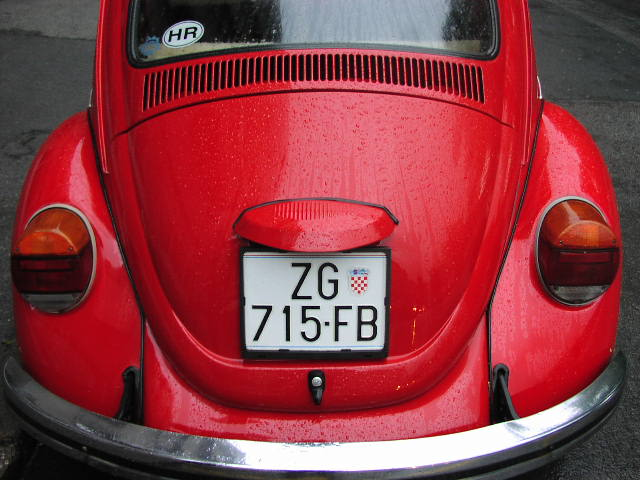
\includegraphics[width=5cm]{P1010013.jpg}
			\caption{Original Image}
		\end{minipage} 
		\begin{minipage}{5cm}
			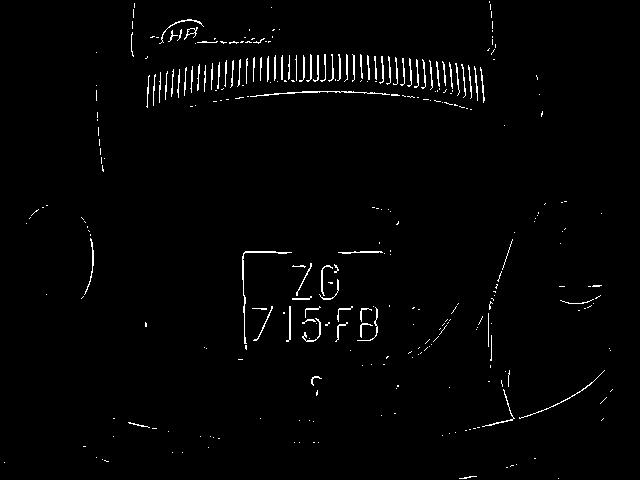
\includegraphics[width=5cm]{P1010013_edge.jpg}
			\caption{After edge detection}
		\end{minipage}
		\begin{minipage}{5cm}
			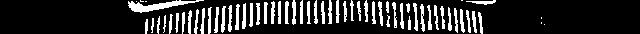
\includegraphics[width=5cm]{P1010013_extract.jpg}
			\caption{After segmentation}
		\end{minipage}
	\end{figure}
	\textbf{Recognition Result: Failed. No character segmentation.}
\end{itemize}


\section{Discussion}
\subsection{Result Anaylsis}
In general, our method does a great job in plate extraction and segmentation and didn't perform very well in the character recognition using CNN. The possible reason can be:
\begin{itemize}
	\item Although the dataset is chosen wisely, there are still quite a few images with relatively poor illumination and strange viewing angles. Our current version doesn't include a rotation-invariant characteristic since the rotation is not in 2-D. Instead it's a projective transformation which requires some techniques in parameters settings. For the illumination, we try to remove shades from the region of interest and it also removes some key information while removing the noises.
	
	\item The relatively poor performance of CNN could attribute to the input images. Since the input images are cropped and segmented by ourselves, it has some differences with the train images EMNIST used by the CNN. For example, 
	\begin{figure}[H]
		\begin{center}
			
\includegraphics[scale=0.6]{confuse_digit.jpg}
			\caption{Confusing digit.}
		\end{center}
	\end{figure}
	The actual digit is '8' while it is quite similar to character 'B'. In such cases, CNN will have a poor performance even with enough training examples.
\end{itemize}

\subsection{Improvements}
\begin{itemize}
	\item Improve the plate extraction and segmentation. We could use some techniques to achieve rotation and illumination invariance which will lead to great improvements in removing noise and extraction. Also, by using some more complex segmentation techniques, we could achieve better segmentation results which will help improve the accuracy.
	
	\item Using R-CNN or other CNN models. Currently we only use CNN at the last stage - recognition. If we could use R-CNN to achieve segmentation and recognition at the same time, the results could be improved. Also, with more accurate and dynamic CNN models (parameters), the recognition could be more robust to confusing characters, which will also help improve the accuracy.
\end{itemize}

\end{spacing}
\bibliography{mytexbib.bib}

\end{document}

